\documentclass[phd,abstract,ackno,listtab,listfig]{wmu-thesis}
\include{packages}
\begin{document}
%% Personal information----------%-------------------------------
\renewcommand{\authname}{Author Name}
\renewcommand{\thesistitle}{\MakeUppercase{Dissertation Title}}
\renewcommand{\gradyear}{2011}
\renewcommand{\gradmonth}{6}
\renewcommand{\departmentname}{Department Name}
\renewcommand{\adviname}{Advisor Name,Ph.D.}
\frontmatter
\mainmatter
\providecommand{\Chapter}[1]{\chapter[\texorpdfstring{\MakeUppercase{#1}}{#1}]{#1}}
%% Main text---------------------%-------------------------------
\Chapter{Introduction}
The quick brown fox jumps over a lazy dog~\cite{Lighthall_2010}.
\begin{figure}[!ht]
\centering
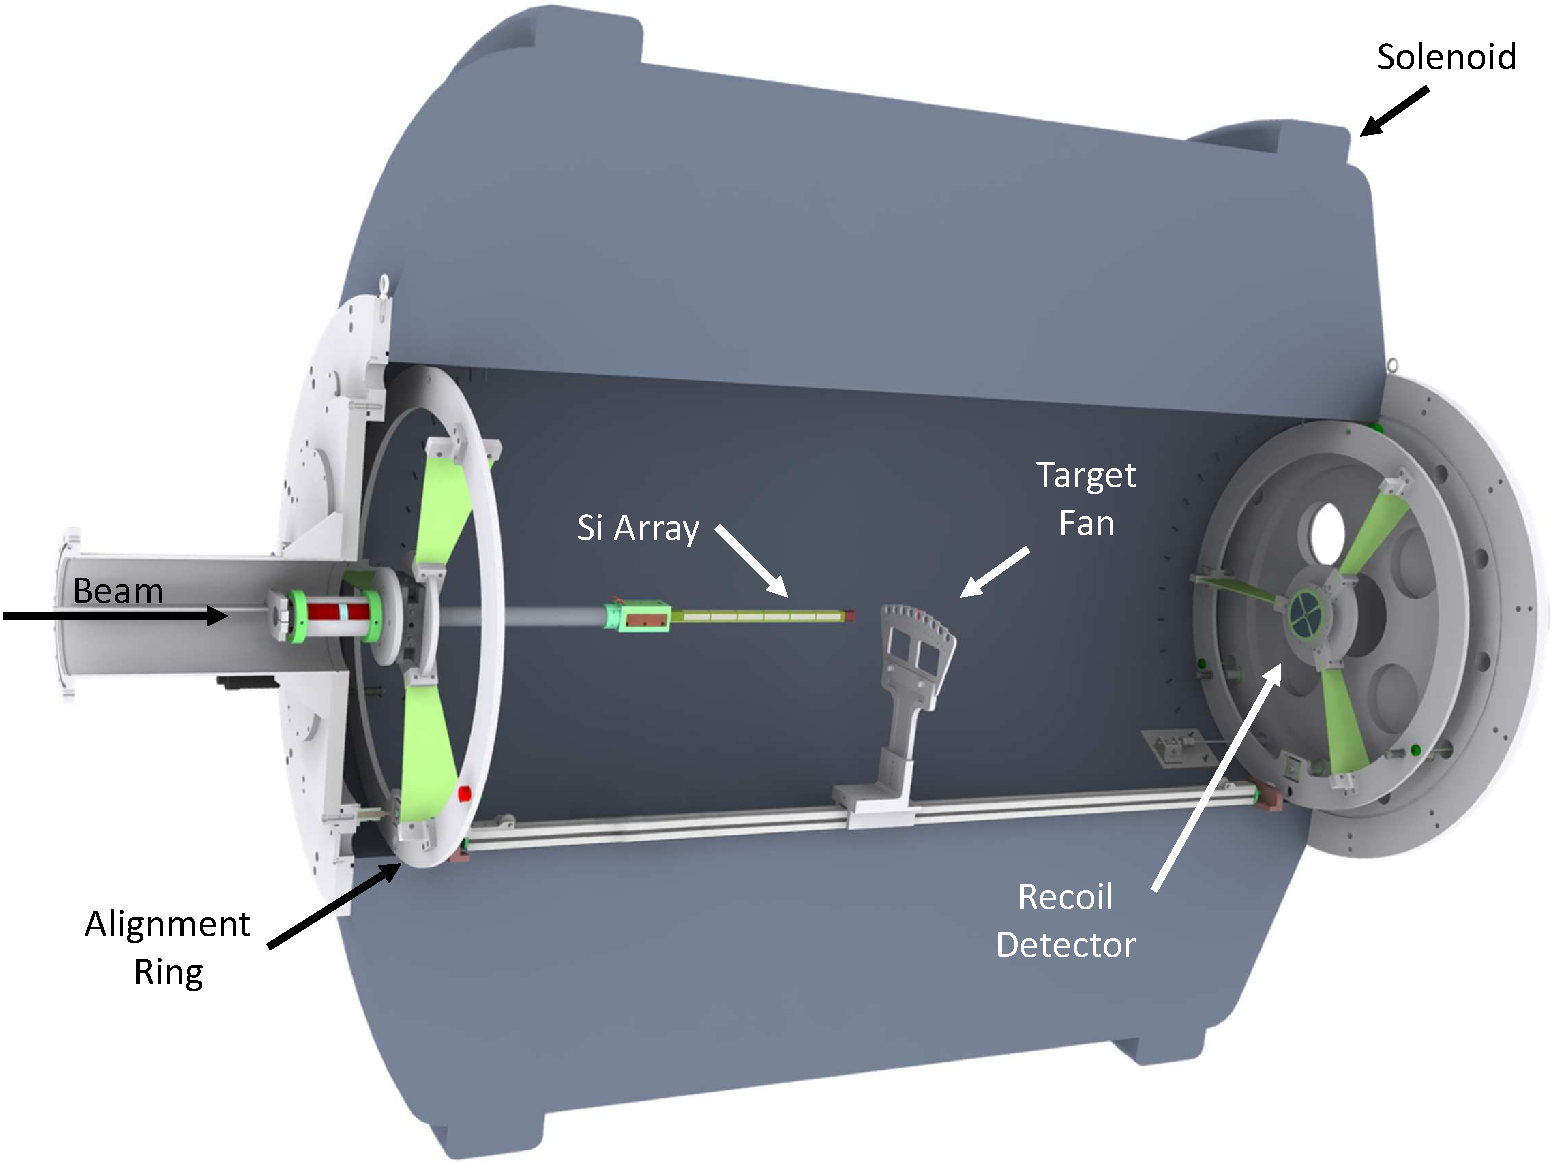
\includegraphics[width=\linewidth,height=0.5\textheight,keepaspectratio]{18pt_rot3}
\caption[Cutaway schematic view of HELIOS in the ``($d$,$p$)'' configuration]{Cutaway schematic view of HELIOS in the ``($d$,$p$)'' configuration.  The accelerated beam enters from left.  Shown are the light-ion silicon detector array suspended on the upstream alignment ring, rotating target fan, and heavy-recoil detector.  Mechanical design by S.~Heimsath.  3D rendering by B.~J.\ DiGiovine.  This figure also appears in Ref.~\cite{Lighthall_2010}.}
\label{schematic}
\end{figure}

%% References--------------------%-------------------------------
\renewcommand{\bibname}{References}%Set the name of the bibliography here
\cleardoublepage
\phantomsection 
\begin{thebibliography}{999}
\bibitem{Lighthall_2010}
J.~C. Lighthall \emph{et~al.}, Nucl.\ Instr.\ and Meth.\ A\textbf{ 622} 97--106 (2010).
\end{thebibliography}
\addcontentsline{toc}{chapter}{\texorpdfstring{\uppercase{\bibname}}{\bibname}}
\twoappendix
\Chapter{Title}
The quick brown fox jumps over a lazy dog.
\end{document}